%\documentclass[unicode]{beamer}
\documentclass[unicode,hyperref={unicode=true}]{beamer}
\mode<presentation>
{
%  \useoutertheme{shadow}
%  \useinnertheme{rounded}
  \usecolortheme[RGB={55,109,160}]{structure}
%  \usetheme[height=7mm]{Rochester}
%  \usetheme{default}
%  \usetheme{Warsaw}
%  \usetheme{Frankfurt}
  \usetheme{Dresden}
%  \setbeamercolor{normal text}{bg=black,fg=white}
  \setbeamertemplate{navigation symbols}{}
  \setbeamertemplate{blocks}[rounded][shadow=true]
  \setbeamertemplate{items}[ball]
  \setbeamercovered{invisible}
}

\defbeamertemplate*{footline}{infolines theme}
{
  \leavevmode%
  \hbox{%
  \begin{beamercolorbox}[wd=\paperwidth,ht=2.25ex,dp=1ex,right]{date in head/foot}%
    \insertframenumber{} / \inserttotalframenumber\hspace*{2ex}
  \end{beamercolorbox}}%
  \vskip0pt%
}

% \setbeamertemplate{headline}{
%   \leavevmode
%  \hbox{%
%  \begin{beamercolorbox}[wd=\paperwidth,ht=3.25ex,dp=1ex,right]{date in head/foot}%
%    Институт системного программирования \\ Российская академия наук
%    \insertframenumber{} / \inserttotalframenumber\hspace*{2ex}
%  \end{beamercolorbox}}%
%  \vskip0pt%
%   \includegraphics[width=\textwidth]{logo-cmb.png}%
%}

\setbeamertemplate{headline}{
	\begin{beamercolorbox}[wd=\paperwidth,ht=3.25ex,dp=1ex,left]{date in head/foot}
		~~\insertsection
	\end{beamercolorbox}
}

\setbeamerfont{section title}{parent=title}
\setbeamercolor{section title}{parent=titlelike}
\defbeamertemplate*{section page kb}{default}[1][]
{
  \centering
	\begin{beamercolorbox}[sep=8pt,center,#1]{section title}
	  \usebeamerfont{section title}\insertsection\par
	\end{beamercolorbox}
}
\newcommand*{\sectionpagekb}{\usebeamertemplate*{section page kb}}
\setbeamercolor{block title}{use=structure,fg=white,bg=structure.fg!75!black}

\usepackage{etex}
\usepackage[T1]{fontenc}
\usepackage[utf8]{inputenc}
\usepackage[russian]{babel}
\usepackage{graphicx}
\usepackage{fancyvrb}
\usepackage{shortvrb}
\usepackage{amsthm}
\usepackage[]{url}
%\MakeShortVerb{!}
\usepackage{listings}
\usepackage{enumerate}
\usepackage{tikz}
\usepackage{xy}
\usepackage{algorithm}
\usepackage{algorithmicx}
\usepackage{algpseudocode}
\usepackage{latexsym}
\usepackage{subfig}
\usepackage{tikz}
\usepackage{dirtree}
\usetikzlibrary{positioning,arrows}
%\lstset{basicstyle=\ttfamily,language=lisp}

\theoremstyle{definition}
\newtheorem{mydef}{Определение}
\theoremstyle{plain}
\newtheorem{stmt}{Утверждение}
%\theoremstyle{plain}
%\newtheorem{lemma}{Лемма}

\title[]
{Автоматизация разработки моделей устройств и вычислительных машин для QEMU}

\author[]{Ефимов Василий}

\institute[]{ИСП РАН}

\date[]{11 октября 2017}

\begin{document}

\begin{frame}
\titlepage
\end{frame}



\begin{frame}{Проблема}
Разработка моделей устройств и вычислительных машин для QEMU~--- это трудоёмкий
процесс. В связи с повысившейся заинтересованностью в расширении QEMU новыми
вычислительными машинами требуется его ускорить. Ускорения предлагается достичь
за счёт автоматизации.
\end{frame}



\begin{frame}{Цели работы}
Целью работы является автоматизация процесса разработки моделей устройств и
вычислительных машин для эмулятора QEMU.

\vskip.5cm

{Для достижения поставленной цели были выполнены следующие задачи:}

\begin{itemize}
\item поиск в исследуемом процессе автоматизируемых этапов;
\item разработка и реализация методов автоматизации;
\item повышение удобства использования реализованного инструмента.
\end{itemize}
\end{frame}



\section{Подход к автоматизации}
\begin{frame}
\sectionpagekb
\begin{itemize}
\item Процесс до автоматизации и его особенности
\item Автоматизированный процесс
\end{itemize}
\end{frame}



\begin{frame}{Процесс разработки до автоматизации}
\begin{center}
\includegraphics[height=0.8\textheight]{workflow-old.png}
\end{center}
\end{frame}



\begin{frame}{Особенности разработки устройства}

\begin{minipage}{0.6\textwidth}

\includegraphics[width=\linewidth]{device-model.png}
\end{minipage}
\begin{minipage}{0.38\textwidth}
\begin{itemize}
\item Развитый обобщающий API
\item Много формального интерфейсного кода
\item Индивидуальный код сосредоточен в чётко определённых местах
\end{itemize}
\end{minipage}

\begin{center}
Можно по краткому перечню параметров сгенерировать сравнительно большую
заготовку.
\end{center}

\end{frame}



\begin{frame}{Особенности разработки ВМ}

\begin{itemize}
\item Декларативный характер определения
\item Применяется объектная модель
\item Сложная система взаимосвязей, тяжело поддающаяся восприятию в форме
программного кода
\end{itemize}

\begin{center}
Можно разработать графический редактор, генерирующий {\it{}почти}
работоспособную модель.
\end{center}

\end{frame}



\begin{frame}{Предлагаемый процесс разработки}
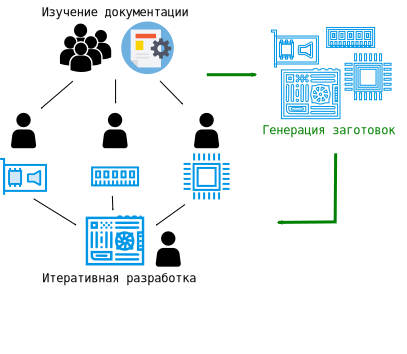
\includegraphics[width=\linewidth]{workflow.png}
\end{frame}



\section{Разработанный инструмент}
\begin{frame}{}
\sectionpagekb
\begin{itemize}
\item Архитектура
\item Возможности
\item Графический интерфейс пользователя (GUI) и API
\item Особенности генерации кода
\item Обратная связь из QEMU
\end{itemize}
\end{frame}{}


\begin{frame}{}
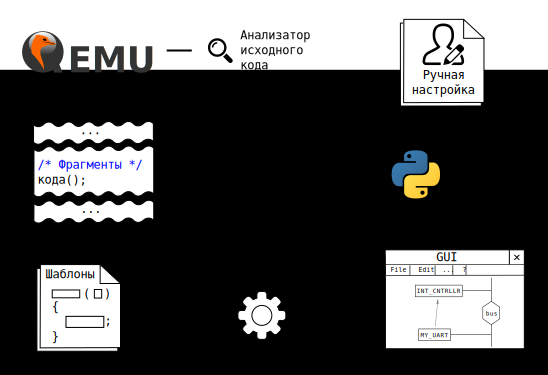
\includegraphics[width=\linewidth]{main.png}
\end{frame}



\begin{frame}{Возможности настройки генерации устройства}
\begin{center}
\begin{tabular}{l|r}
Класс устройства & Настройки \\
\hline
Любой            & таймеры \\
                 & символьные и блочные устройства \\
                 & сетевой интерфейс \\
\hline
Устройство       & MMIO \\
системной        & PMIO \\
шины             & in/out IRQ \\
\hline
Функция          & BAR \\
PCI(E)           & out IRQ (INTx) \\
устройства       & MSI(X) \\
                 & идентификационная информация
\end{tabular}
\end{center}
\end{frame}



\begin{frame}{GUI настройки генерации устройства}
\begin{center}
PCI Fast Ethernet контроллер из С2600
\end{center}
\includegraphics[width=\linewidth]{AM79C971.jpg}
\end{frame}



\begin{frame}[fragile]{Код настройки генерации устройства}

\lstset{language=Python}
\begin{lstlisting}
obj43 = SysBusDeviceDescription(
    name = "CISCO remote",
    directory = "char",
    out_irq_num = 0,
    in_irq_num = 0,
    mmio_num = 0x1,
    pio_num = 0,
    nic_num = 0,
    timer_num = 0,
    char_num = 0x1,
    block_num = 0x1
)
\end{lstlisting}

\end{frame}



\begin{frame}[fragile]{API компоновки вычислительной машины}

\dirtree{%
.1 Node .
    .2 BusNode .
        .3 SystemBusNode .
        .3 PCIExpressBusNode .
        .3 [ISA, IDE, I2C]BusNode .
    .2 DeviceNode .
        .3 SystemBusDeviceNode .
        .3 PCIExpressDeviceNode .
    .2 IRQLine .
    .2 IRQHub .
    .2 MemoryNode .
        .3 MemoryLeafNode .
            .4 MemoryAliasNode .
            .4 MemoryRAMNode .
            .4 MemoryROMNode .
}
\end{frame}



\begin{frame}{Схема вычислительной машины}
\begin{minipage}[b]{0.71\textwidth}
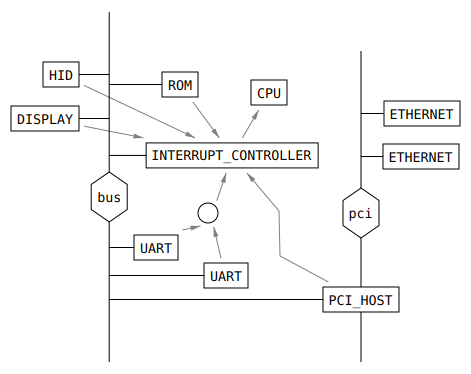
\includegraphics[width=\linewidth]{machine-example.png}
\vfill
\end{minipage}
\hfill
\begin{minipage}[t]{0.24\textwidth}
\vfill
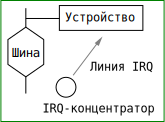
\includegraphics[width=\linewidth]{legend.png}
\end{minipage}
\end{frame}



\begin{frame}{GUI настройки интеграции устройства}
\includegraphics[height=0.9\textheight]{REMOTE.jpg}
\end{frame}



\begin{frame}[fragile]{Код настройки интеграции устройства}

\lstset{language=Python}
\begin{lstlisting}
obj3 = SystemBusDeviceNode(
    qom_type = "TYPE_CISCO_REMOTE",
    system_bus = obj1,
    mmio = [ 0xf6000000 ]
)
obj3.properties.extend([
    QOMPropertyValue(QOMPropertyTypeString,
        "chardev", "serial2"),
    QOMPropertyValue(QOMPropertyTypeString,
        "eeprom_c2600_mb", "eeprom-c2600-mb"),
    QOMPropertyValue(QOMPropertyTypeLink,
        "nvram", obj2),
    QOMPropertyValue(QOMPropertyTypeInteger,
        "remote_cpu_type", 0x2)
])
\end{lstlisting}

\end{frame}



\begin{frame}{Требования к генерируемому коду:}
\begin{itemize}
\item синтаксическая корректность~--- возможность сразу после генерации
сосредоточиться на написании индивидуальной части кода;
\begin{itemize}
\item подключены все заголовки;
\item правильный порядок фрагментов кода;
\end{itemize}
\item соответствие стилю программирования~--- минимизация количества времени,
требуемого на последующий рефакторинг;
\begin{itemize}
\item соблюдены отступы и правила переноса;
\item соблюдены соглашения об именовании символов;
\item семантическая группировка фрагментов кода.
\end{itemize}
\end{itemize}
\end{frame}



\begin{frame}{Устройство генератора}
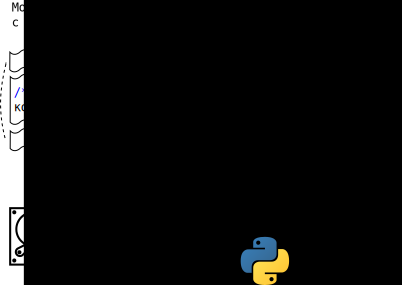
\includegraphics[height=0.9\textheight]{generation.png}
\end{frame}



\begin{frame}{Модель языка программирования}
\dirtree{%
.1 object .
    .2 Source\ \ \ \ \ \ \ \ \ \ \ \ \ - контейнер.
        .3 Header.
    .2 Type .
        .3 Structure\ \ \ \ \ \ \ - для Си.
        .3 Function .
        .3 Pointer .
        .3 Enumeration .
        .3 Macro\ \ \ \ \ \ \ \ \ \ \ - для препроцессора.
        .3 TypeReference\ \ \ - межфайловая связь.
    .2 Variable\ \ \ \ \ \ \ \ \ \ \ - Type + имя.
    .2 Initializer\ \ \ \ \ \ \ \ \ \ \ \ \{ + начальное значение \}.
    .2 Usage\ \ \ \ \ \ \ \ \ \ \ \ \ \ - Type/Variable + Initializer.
}
\end{frame}



\begin{frame}{Пример модели исходного кода}
Устройство с одним регистром\\
\vfill
\begin{center}
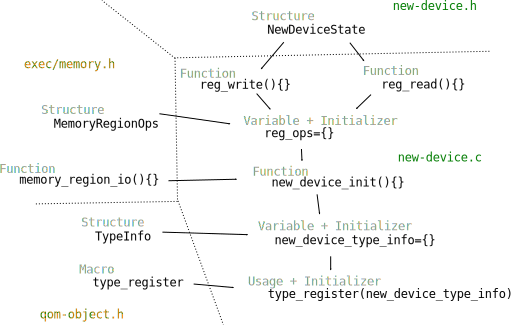
\includegraphics[height=0.75\textheight]{source-example.png}
\end{center}
\end{frame}



\begin{frame}{Модель файла с исходным кодом}
\begin{minipage}{0.61\textwidth}
\includegraphics[width=\linewidth]{c2600_pci_c_chunks.png}
\end{minipage}
\begin{minipage}{0.37\textwidth}
\begin{itemize}
\item Топологическая сортировка
\item Семантическая сортировка
\item Оптимизация количества включаемых заголовков (транзитивное сокращение
графа включения)
\end{itemize}
\end{minipage}
\end{frame}



\begin{frame}{Анализ QEMU, взаимосвязь}
\begin{minipage}{0.35\textwidth}
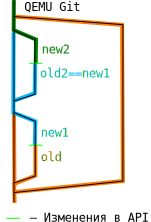
\includegraphics[height=0.8\textheight]{heuristics.png}
\end{minipage}
\hfill
\begin{minipage}{0.63\textwidth}
\begin{itemize}
\item Автоматический анализ заголовков QEMU
    \begin{itemize}
    \item Граф включения
    \item Макросы
    \end{itemize}
\item Эвристическая адаптация к изменениям API QEMU с привязкой к истории Git
\end{itemize}
\end{minipage}
\end{frame}



\section{Примеры применения инструмента}
\begin{frame}
\sectionpagekb
\begin{itemize}
\item PC на базе Intel Q35
\item Криптомаршрутизатор СISCO серии 2600 (C2621XM)
\end{itemize}
\end{frame}



\begin{frame}{PC на базе Intel Q35}
\begin{itemize}
\item Реализация Q35 уже имеется в QEMU и является одной из самых сложных.
\item Цель эксперимента~--- убедиться в эквивалентности предельных возможностей
предлагаемого метода (по сравнению с классическим, ручным).
\item Многие устройства в QEMU уже присутствовали.
\item Остальные были реализованы в соответствии с действующими требованиями
QEMU при помощи инструмента.
\end{itemize}
\end{frame}



\begin{frame}{}
\begin{center}
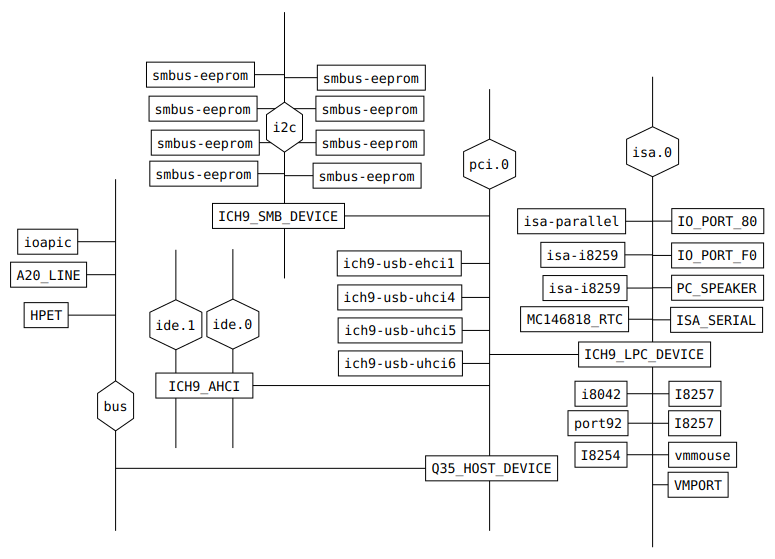
\includegraphics[height=\textheight]{Q35-h.png}
\end{center}
\end{frame}



\begin{frame}{Статистика*}
\begin{center}
\begin{tabular}{l|lll}
Этап         & Затронуто & Вставлено & Удалено \\
             & файлов    & строк     & строк   \\
\hline
Подготовка** & 4         & 42        & 31      \\
Генерация    & 8         & 599       & 0       \\
Реализация   & 5         & 142       & 93***   \\
Суммарно     & 12        & 789       & 31      \\
\end{tabular}
\end{center}
\vfill
\it{*Статистика собрана с помощью git diff.}\\
\it{**Перенос необходимых символов в заголовочные файлы,
объявление глобальных переменных.}\\
\it{***Количество удаленных при реализации строк близко к количеству строк,
которые потребовалось исправить в сгенерированном коде.}
\end{frame}



\begin{frame}{Криптомаршрутизатор С2600 (C2621XM)}
\begin{itemize}
\item За основу взята реализация из Dynamips.
\item CPU PowerPC MPC860 изначально реализован без поддержки полносистемной
эмуляции.
\item Машина и все устройства (кроме CPU) были реализованы с помощью
инструмента.
\end{itemize}
\end{frame}



\begin{frame}{Схема C2621XM}
\begin{center}
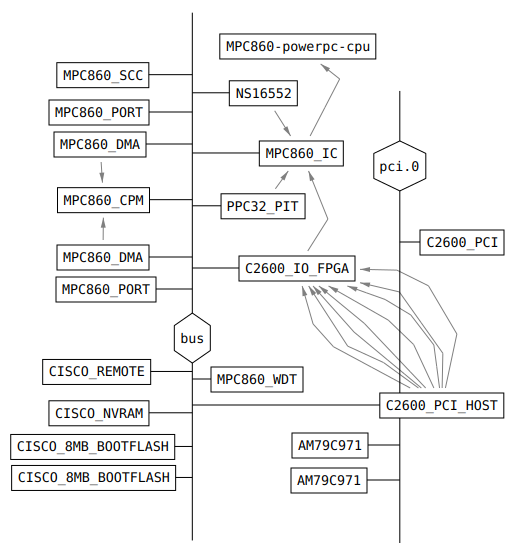
\includegraphics[height=0.8\textheight]{C2600.png}
\end{center}
\end{frame}



\begin{frame}{Статистика}
\begin{center}
\begin{tabular}{l|lll}
Этап         & Затронуто & Вставлено & Удалено \\
             & файлов    & строк     & строк   \\
\hline
Подготовка*  & 8         & 128       & 35      \\
Генерация    & 37        & 2186      & 0       \\
Реализация   & 31        & 4747      & 419     \\
Суммарно     & 45        & 6642      & 35      \\
\end{tabular}
\end{center}
\vfill
\it{*MMU, спец. регистры и прерывания CPU, идентификаторы PCI.}
\end{frame}



\begin{frame}{Статистика*}
\begin{center}
\begin{tabular}{l|ll}
Устройство        & Объём конфигурации & Сгенерировано \\
\hline
MPC860\_IC        & 6                  & 125           \\
C2600\_PCI\_HOST  & 6                  & 133           \\
C2600\_PCI        & 7                  & 82            \\
NS16552           & 7                  & 181           \\
C2600\_IO\_FPGA   & 8                  & 137           \\
CISCO\_REMOTE     & 7                  & 152           \\
AM79C971          & 12                 & 175           \\
\end{tabular}
\end{center}
\vfill
\it{*Объём кода приведён в строках.}
\end{frame}



\section{Результаты}
\begin{frame}
\sectionpagekb
\vfill
\begin{itemize}
\item Автоматизирован начальный этап разработки машины и устройства
\item Настройка генерации осуществляется на языке Python
\item Объём настройки генерации заготовки устройства в 11-25 раз меньше объёма
сгенерированной заготовки
\item Разработан GUI, в т.ч. с визуализацией машины в виде схемы
\item Поддерживается разработка машин, сравнимых по сложности с Intel Q35
\item Доля сгенерированного кода составляет от \(1/4\) до \(3/4\) в зависимости
от количества уже реализованных устройств
\item Реализована обратная связь из QEMU
\end{itemize}
\end{frame}



\begin{frame}
\begin{center}
Спасибо за внимание
\end{center}
\end{frame}



\end{document}
